% !TeX spellcheck = de_DE
\documentclass{alex_hü}

\usepackage{float}

\name{Alexander Helbok}
\course{Praktische Astronomie}
\hwnumber{1}

\chead{\textbf{\Large Mondcheck}}

\begin{document}
%\renewcommand{\labelenumi}{\alph{enumi})}


\begin{enumerate}
	\item \textbf{Wie groß ist der Mond im Vergleich zur Erde? \\}
	Der Radius des Mondes beträgt \( R_m = 1737 \unit{km} \), was 3.7 mal kleiner als der der Erde ist. Betrachtet man das Volumen (das mit \( r^3 \) skaliert) ist der Mond um 50 mal kleiner als die Erde.
	
	\textbf{\item Warum hat der Mond keine Atmosphäre? \\} 
	Der Mond ist zu leicht, um eine Atmosphäre gravitativ zu binden. Zudem würde diese vom Sonnenwind weggeblasen werden, da der Mond kein starkes Magnetfeld besitzt	
	
	\textbf{\item Wie lange braucht ein Laserstrahl in etwa von der Erde zum Mond und retour?  \\}
	Der Mond ist \( 405000 \unit{km} \) von uns entfernt, was eine Lichtlaufzeit von \( 1.35 \unit{s} \) ausmacht. Ein Laserstrahl braucht also \( 2.7 \unit{s} \), um von der Erde zum Mond und wieder zurück zu kommen.
	
	\textbf{\item Was versteht man unter „gebundener Rotation“ des Mondes?  \\}
	Der Mond zeigt der Erde immer die gleiche Seite, da die Rotationen von Mond und Erde aufeinander abgestimmt sind
	
	\textbf{\item Was ist der Unterschied zwischen einem siderischen und einem synodischen Monat?  \\}
	Der siderische Monat wird in einem fixen Bezugssystem gemessen und ist die Zeit die der Mond braucht, um wieder am gleichen Fleck zwischen den Fixsternen zu erreichen. Der synodische Monat hingegen gibt an, wann der Mond wieder die gleiche Mondphase erreicht hat, was etwas länger als der siderische Monat ist, da die Erde um die Sonne läuft und der Mond daher etwas Entfernung “aufholen” muss.
	
	\textbf{\item Warum gibt es auf dem Mond keine Jahreszeiten?  \\}
	Ohne Atmosphäre sind Wetter und Jahreszeit schwer zu definieren; Temperaturschwankungen sind am Mond zu beobachten, aber Wetterphänomene die wir mit Jahreszeiten verbinden gibt es am Mond nicht.
	
	\textbf{\item Nennen Sie fünf Mond-Mare. 8. Wo befinden sich diese Mare? Versuchen Sie, ihre Lage zu beschreiben.  \\}
	Die Namen von fünf Mond-Mare sind Mare Serenitatis, Mare Tranquillitatis, Mare Imbrium, Mare Nubium und Mare Procellarum.
	
	\textbf{\item Wie sind die Mare entstanden und warum sind sie relativ dunkel?  \\}
	Mare sind Krater von eingeschlagenen Meteoriten, in welche sich Lava aus einer früheren, von Vulkanismus gepräten Phase des Mondes angesammelt hat.
	
	\textbf{\item Wie heißen einige der Mondkrater, die Sie beobachtet haben?  \\}
	Fracastorius, Manilus, Taruntius, Posidonius, Aristoteles
	
	\textbf{\item Wo befinden sich diese Krater in Bezug auf die Mare? \\}
	Krater befinden sich meistens am Rande eines Mares
	
	\textbf{\item Was befindet sich manchmal in der Mitte eines Mondkraters und wie ist es entstanden? \\}
	Ein zentraler Gipfel, der als Überlagerung von Schockwellen entsteht.
	
	\textbf{\item Wie kann man sich die von Mondkratern ausgehenden Strahlensysteme erklären?  \\}
	Beim Einschlag von Meteoriten können je nach Einschlagswinkel Teile des Meteoriten radial nach außen geschleudert werden.
	
	\textbf{\item Was fällt bei der Namensgebung der Mare, Krater und Gebirge auf?  \\}
	Mare sind nach leitischen Begriffen,Krater nach Persönlichkeiten und Gebirge nach Orten auf der Erde benannt

	\textbf{\item Wie bezeichnet man auch dem Mond die Grenze zwischen Tag und Nacht?  \\}
	Terminator
	
	\textbf{\item Welche Temperaturen herrschen am Mondtag (Sonne im Zenit) bzw. in der Mondnacht?
	(Die erste Mondlandung am 20.7.1969 fand einen Tag nach Sonnenaufgang statt.)  \\}
	Die Extrema der Temperatur am Mond betragen \( -133 \unit{\celsius} \) in der Nacht und \( 121 \unit{\celsius} \) unter Tags
	
	\textbf{\item Wie viele Menschen haben den Mond bisher betreten (zwei pro Landung)?  \\}
	12 Menschen haben den Mond betreten
	
	\textbf{\item Wie viele bemannte Apollo-Mondlandungen gab es daher?  \\}
	Es hab daher 6 Apollo Missionen mit erfolgreicher Mondlandung
	
	\textbf{\item Was versteht man unter Libration des Mondes?  \\}
	Der Mond scheint von der Erde aus gesehen zu taumeln, da dieser keine perfekte Kreisbahn verfolgt, und wir daher nicht immer 
	
	\textbf{\item Welche Bahn beschreibt die Erde scheinbar am Mondhimmel? \\}
	Da die Rotation des Mondes an die Erde gebunden ist, erscheint die Erde am Mond als statischer Punkt
	
	\textbf{\item Warum ist der Vollmond nicht doppelt so hell wie der Halbmond?  \\}
	Bei Vollmond erhalten wir auf der Erde (fast) die gesamte Strahlung die den Mond trifft zurückreflektiert, während bei Halbmond der großteil ins All zurückreflektiert wird und nur wenig seitlich zur Erde hin reflektiert wird.
	
	\textbf{\item Welche aktiven Raumsonden befinden sich derzeit auf dem Mond?  \\}
	Derzeit befinden sich keine Raumsonden auf der Mondoberfläche
	
	\textbf{\item Bestimmen Sie mittels eines der folgenden Bilder die Größe des Erdschattenradius im Vergleich zum Mondradius, d.h. um welchen Faktor ist der Erdschattenradius größer als der Mondradius? \\}
	Um den Radius der Erde zu bestimmen wurde das Bild in ein CAD Programm (Fusion 360) importiert. Dieses kann man dann als Vorlage verwenden um 3 Punkte auf dem Bild zu markieren, woraus sich ein eindeutiger Kreis konstruieren lässt. Vergleicht man die Beiden Radien, sieht man dass der Schatten der Erde etwas mehr als doppelt so groß ist, wie der des Mondes. 
	
	\begin{figure}[H]
		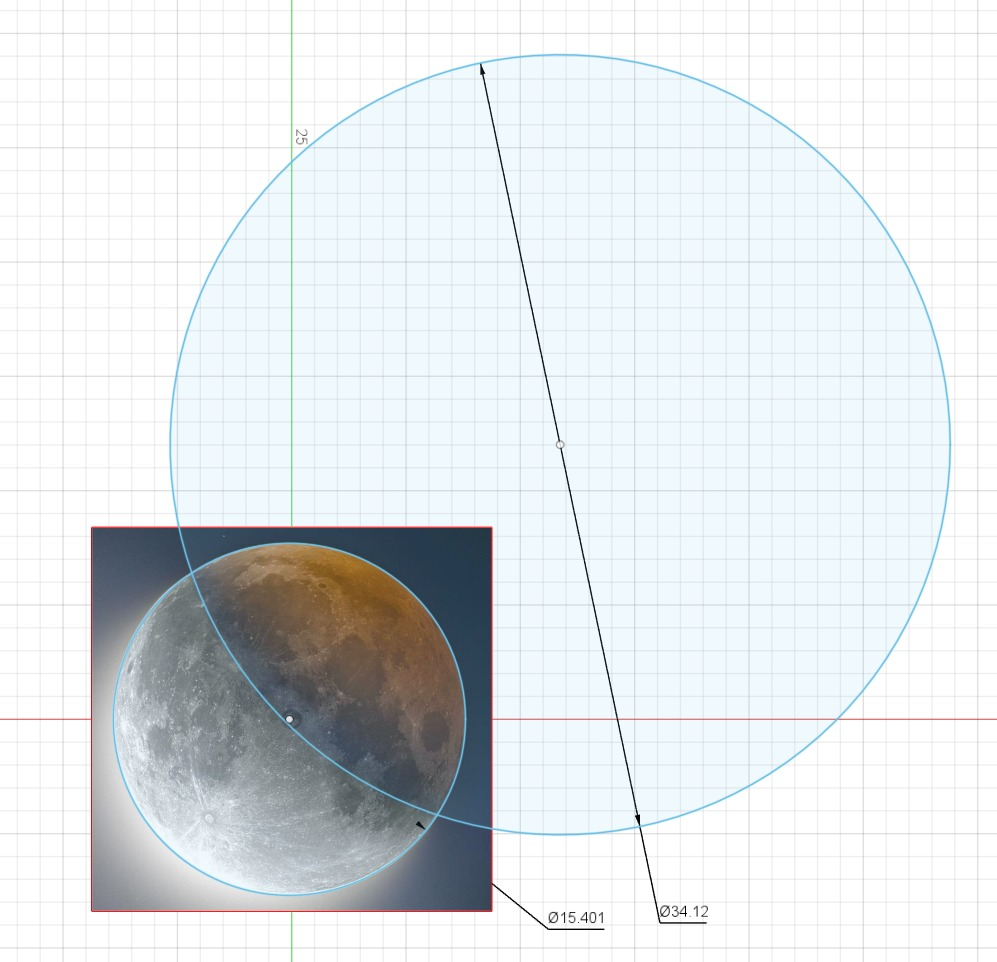
\includegraphics[scale=0.3]{fusion}
	\end{figure}
	
\end{enumerate}

\end{document}